\documentclass[../main.tex]{subfiles}
\begin{document}
\chapter{The Double-$\tau_h$ + jet trigger}

In view of Run 3, a lot of effort has been dedicated in order to maximize the collection efficiency from rare physics processes. In our case, we will try to increase the acceptance to the $H\to\tau\tau$ and $HH\to bb\tau\tau$ processes.

In most of the $H\to\tau\tau$ events used in the analysis, the $\tau\tau$ pair is accompanied by one or more jets coming from the hard-scattering processes or from QCD radiation (in addition to the 2 $b$-jets coming from the other $H$ in the $HH\to bb\tau\tau$ analysis). In fact, as shown in Fig. \ref{hh:fig:trig_htt_acc}, most of the sensitivity in the $H\to\tau\tau$ analysis \cite{hh:htt_2016} comes from the boosted (1 jet) and VBF (2 jets) categories. Therefore, the acceptance of both analysis could be enlarged by requiring at trigger level an additional jet to the already present double-$\tau_h$ trigger so the $p_t$ thresholds on the $\tau_h$ candidates can be lowered.


\begin{figure}[h!]
\begin{center}
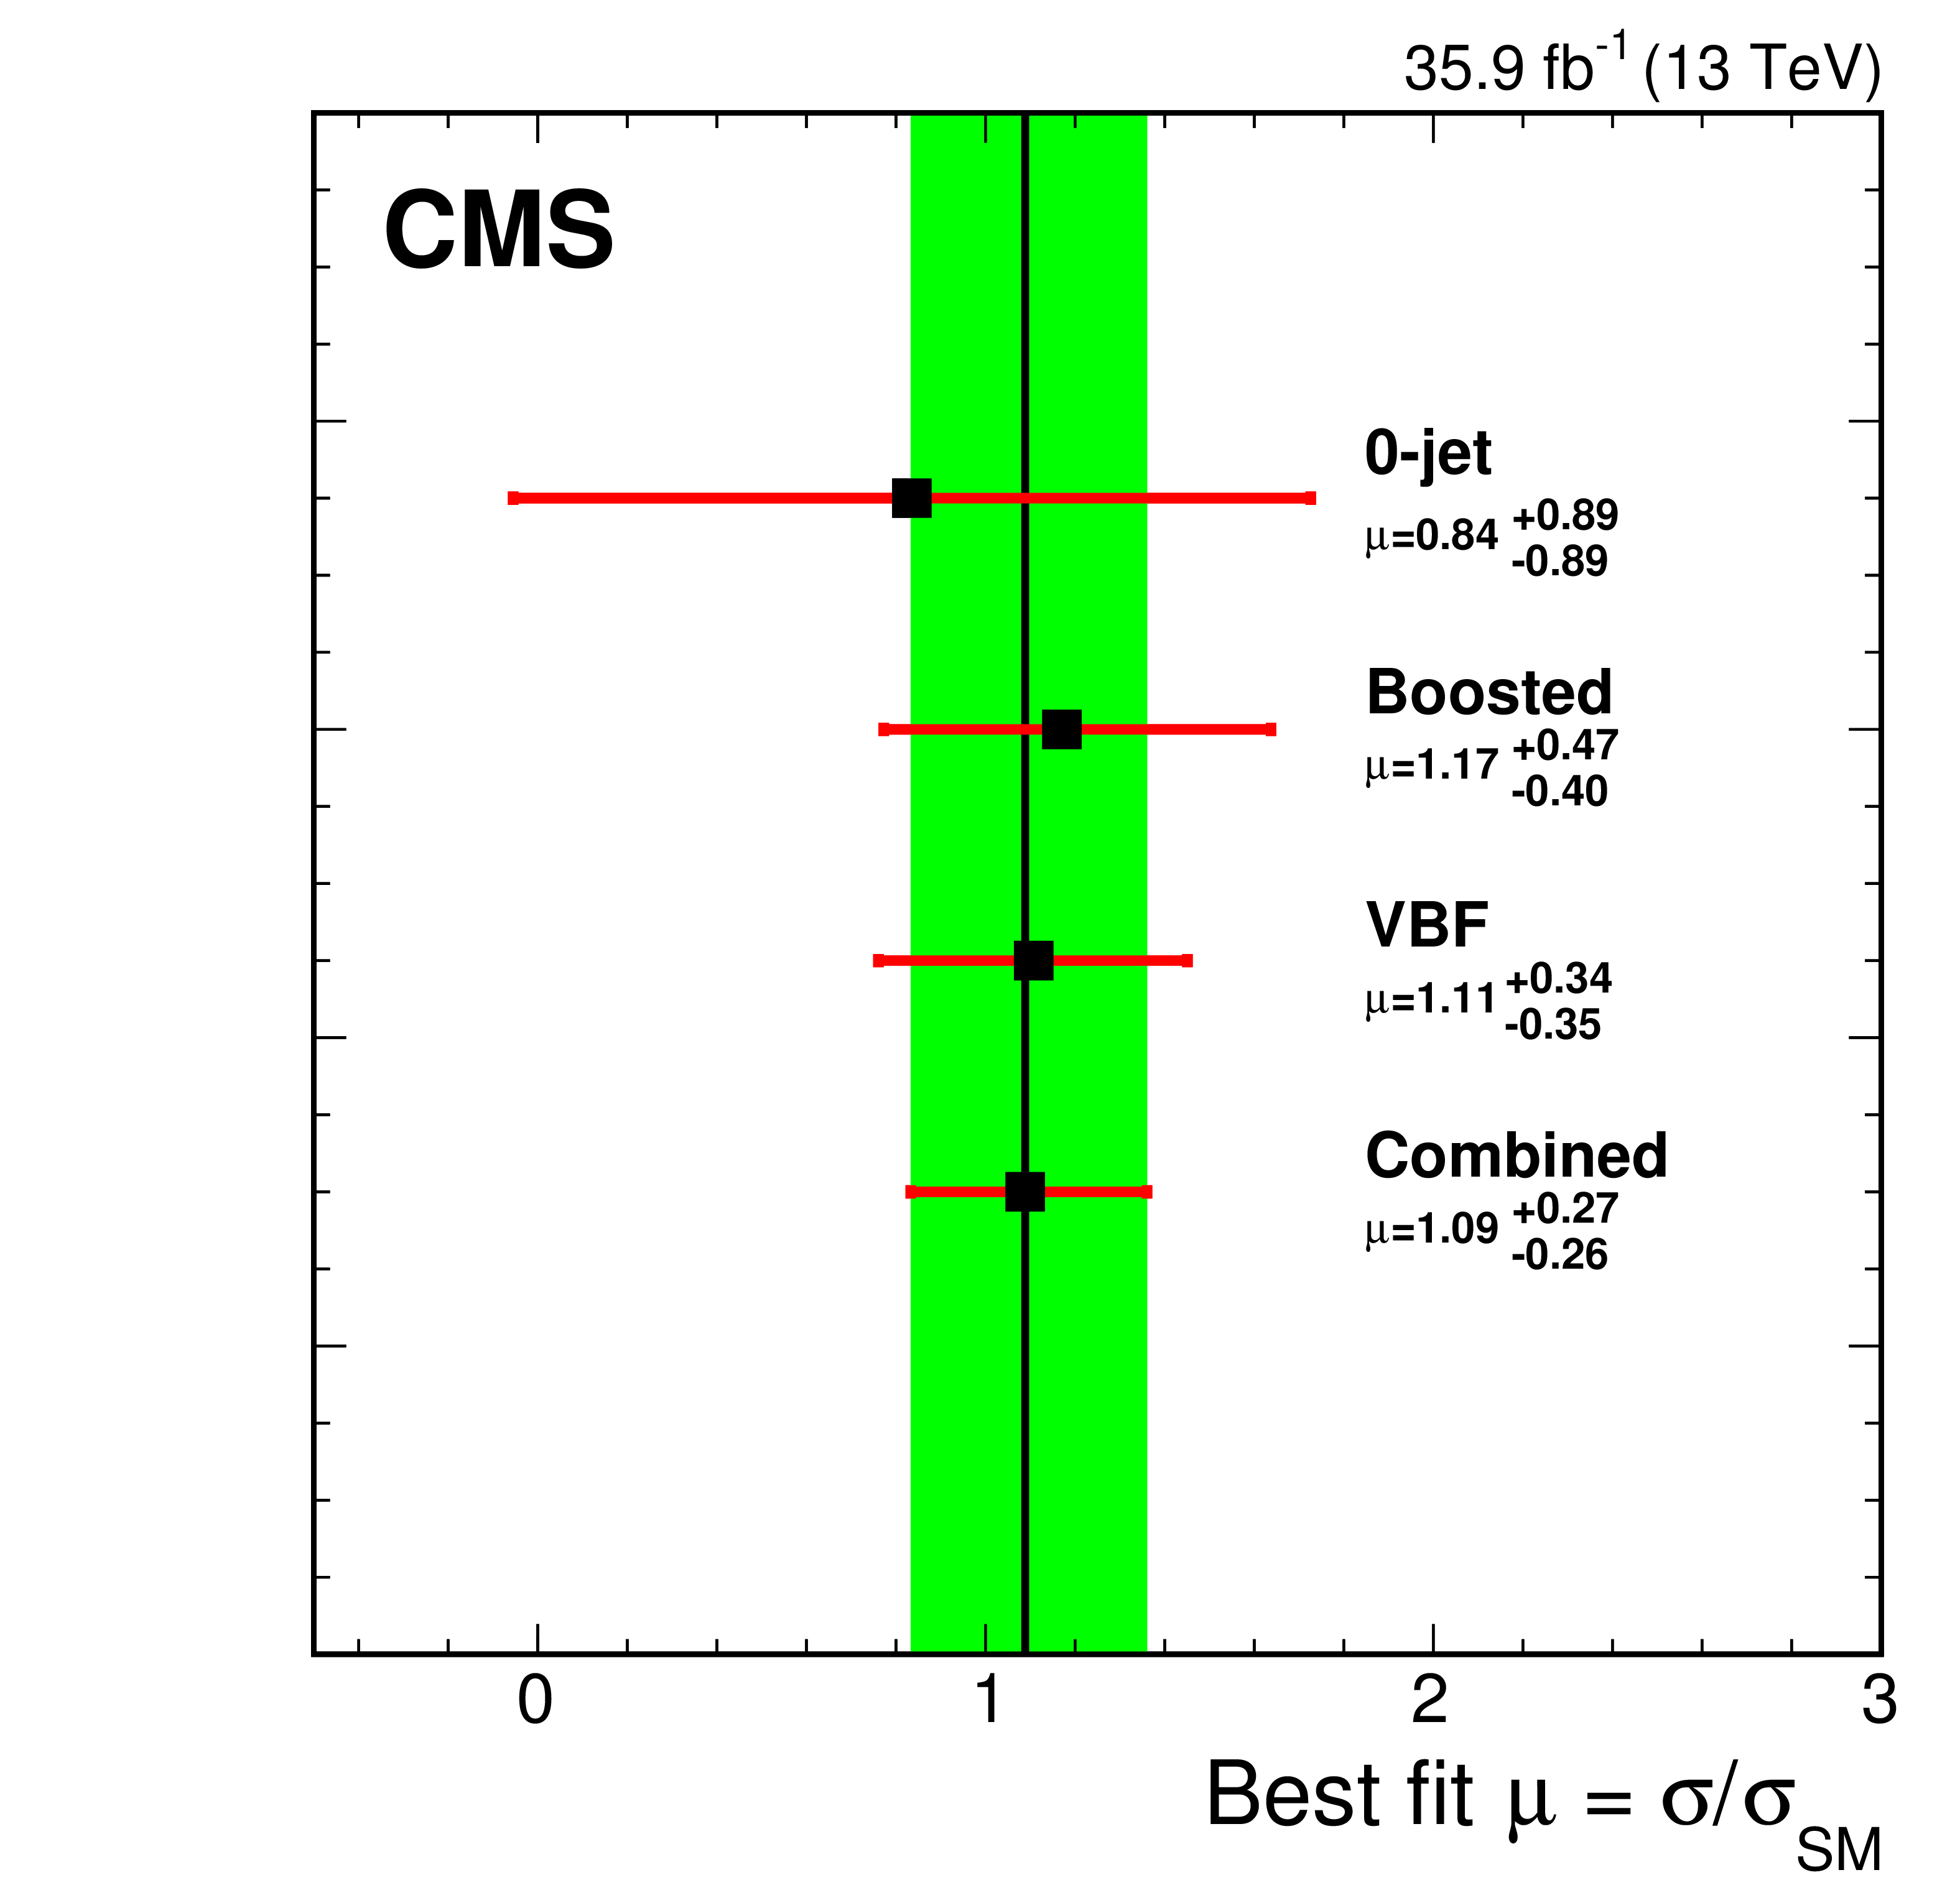
\includegraphics[width=0.5\textwidth]{Images/CMS-HIG-16-043_Figure_021-a.png}
\end{center}
\caption{Best fit $H\to\tau\tau$ signal strength per analysis category.}
\label{hh:fig:trig_htt_acc}
\end{figure}



\section{The L1 Double-$\tau_h$ + jet(s) trigger(s)}

\textcolor{red}{Shall we explain here L1 menu or in the introduction?}

At L1, the strategy followed was to include one or two seeds in the L1 Menu with two isolated $\tau_h$ objects and one or two jet objects identified by the $\mu$GT in order to complement the already present \texttt{L1\_DoubleIsoTau32er2p1} seed, where two isolated $\tau_h$ with $p_t\geq32$~GeV and $|\eta|<2.1$ are considered. However, a particular treatment has to be given to seeds involving $\tau_h$ and jet objects simultaneously, as both are reconstructed as purely calorimetric objects. Then, all $\tau_h$ objects will enter the L1 jet collection, while some of the L1 jets will appear in the L1 $\tau_h$ collection. To reduce this effect, a feature called overlap removal \cite{intro:l1_13tev} is used,  so only L1 jets that are more than $\Delta R>0.5$ with the selected $\tau_h$ are considered. This feature was present in the $\mu$GT before the inclusion of the seeds, although none of the already present seeds were using it and, in fact, it had to be tuned before attempting the inclusion of the new seeds. Therefore, the seeds we will consider and study will have the structure \texttt{L1\_DoubleIsoTauXer2p1\_JetY\_RmOvlp\_dR0p5} for single-jet seeds and \texttt{L1\_DoubleIsoTauXer2p1\_JetY\_RmOvlp\_dR0p5\_JetZ\_RmOvlp\_dR0p5} and \texttt{L1\_DoubleIsoTauXer2p1\_DoubleJetY\_RmOvlp\_dR0p5} for double-jet seeds with asymmetric and symmetric $p_t$ thresholds for the jets respectively.

To evaluate the performance of the new seeds, two quantities are considered. First, as we would like to increase the signal acceptance, we compute the acceptance gain with the new seeds with respect to the reference \texttt{L1\_DoubleIsoTau32er2p1} seed considering four signal samples, two ggH and VBFH $H\to\tau\tau$ and two ggHH and VBFHH $HH\to bb\tau\tau$. These acceptance gains are computed not only considering if the L1 objects pass the required selection cuts, but also applying selections to the objects obtained by the offline reconstruction system that evolve accordingly to the L1 thresholds considered. In general, this evolution means that, for a given L1 $p_t$ threshold X, the offline threshold is obtained as X + $\Delta X$, where $\Delta X>0$ is a quantity that will depend on the analysis considered. For instance, in the $H\to\tau\tau$ analysis \cite{hh:htt_2016}, the leading $\tau_h$ is required to have a $p_t\geq 50$~GeV, while for the subleading this value drops to 40~GeV. Therefore, we will consider $\Delta X=18$ GeV and $\Delta X=8$ GeV for the leading and subleading $\tau_h$ respectively when obtaining the $H\to\tau\tau$ acceptance gains. In the $HH\to bb\tau\tau$ analysis \textcolor{red}{[paper when it's ready]} both $\tau_h$ are required to have a $p_t\geq40$~GeV, so we will set $\Delta X=8$~GeV for both $\tau_h$. For the jets, we will consider $\Delta X=10$~GeV for both analysis. Apart from this $p_t$ requirements, two different categorizations will be applied to the $H\to\tau\tau$ samples and one to the $HH\to bb\tau\tau$. Among the first ones we find the 1-jet, High pt category, where we consider events with a $\geq70$~GeV jet, and the 2-jet category, where we ask for two $\geq30$~GeV jets. In the \textbf{$bb\tau\tau$} category we will just ask for 2 jets with $p_t\geq20$~GeV. All $p_t$ selections are summarised in Table~\ref{hh:tab:trig_offpt}, where one boolean to each of the seeds considered has been defined to group the associated selections. On top of these $p_t$ cuts, we ask all offline jets to have $|\eta|<4.7$ and pass tight jet ID and loose PU jet ID and an overlap removal criteria with the offline $\tau_h$.




\begin{table}
	\begin{center}
	\begin{tabular}{c || c | c | c }
		                           & \multicolumn{3}{c}{Offline selections} \\
		Boolean                    & 1-jet, high $p_t$ & 2-jet & bb$\tau\tau$ \\\hline\hline
		\texttt{PassOfflDoubleTau32} & 
			$\begin{matrix}
				p_t^{\tau_1}>50\\
				p_t^{\tau_2}>40\\
				p_t^{j_1}>70
			\end{matrix}$ &
			$\begin{matrix}
				p_t^{\tau_1}>50\\
				p_t^{\tau_2}>40\\
				p_t^{j_1}>30 \\
				p_t^{j_2}>30
			\end{matrix}$ &
			$\begin{matrix}
				p_t^{\tau_1}>50\\
				p_t^{\tau_2}>40\\
				p_t^{j_1}>20\\
				p_t^{j_2}>20
			\end{matrix}$ \\\hline
		\texttt{PassOfflDoubleTauXJetY} &
			$\begin{matrix}
				p_t^{\tau_1}>X+18\\
				p_t^{\tau_2}>X+8\\
				p_t^{j_1}>Y+10 \\
				p_t^{j_1}>70
			\end{matrix}$ &
			$\begin{matrix}
				p_t^{\tau_1}>X+18\\
				p_t^{\tau_2}>X+8\\
				p_t^{j_1}>Y+10 \\
				p_t^{j_1}>30 \\
				p_t^{j_2}>30
			\end{matrix}$ &
			$\begin{matrix}
				p_t^{\tau_1}>X+8\\
				p_t^{\tau_2}>X+8\\
				p_t^{j_1}>Y+10 \\
				p_t^{j_1}>20 \\
				p_t^{j_2}>20
			\end{matrix}$ \\\hline
		\texttt{PassOfflDoubleTauXJetYJetZ} &
			$\begin{matrix}
				p_t^{\tau_1}>X+18\\
				p_t^{\tau_2}>X+8\\
				p_t^{j_1}>Y+10 \\
				p_t^{j_1}>70 \\
				p_t^{j_2}>Z+10 \\
			\end{matrix}$ &
			$\begin{matrix}
				p_t^{\tau_1}>X+18\\
				p_t^{\tau_2}>X+8\\
				p_t^{j_1}>Y+10 \\
				p_t^{j_1}>30 \\
				p_t^{j_2}>Z+10 \\
				p_t^{j_2}>30 
			\end{matrix}$ &
			$\begin{matrix}
				p_t^{\tau_1}>X+8\\
				p_t^{\tau_2}>X+8\\
				p_t^{j_1}>Y+10 \\
				p_t^{j_1}>20 \\
				p_t^{j_2}>Z+10 \\
				p_t^{j_2}>20
			\end{matrix}$ \\\hline
		\texttt{PassOfflDoubleTauXDoubleJetY} &
			$\begin{matrix}
				p_t^{\tau_1}>X+18\\
				p_t^{\tau_2}>X+8\\
				p_t^{j_1}>Y+10 \\
				p_t^{j_1}>70 \\
				p_t^{j_2}>Y+10 \\
			\end{matrix}$ &
			$\begin{matrix}
				p_t^{\tau_1}>X+18\\
				p_t^{\tau_2}>X+8\\
				p_t^{j_1}>Y+10 \\
				p_t^{j_1}>30 \\
				p_t^{j_2}>Y+10 \\
				p_t^{j_2}>30 
			\end{matrix}$ &
			$\begin{matrix}
				p_t^{\tau_1}>X+8\\
				p_t^{\tau_2}>X+8\\
				p_t^{j_1}>Y+10 \\
				p_t^{j_1}>20 \\
				p_t^{j_2}>Y+10 \\
				p_t^{j_2}>20
			\end{matrix}$
	\end{tabular}
	\end{center}

	\caption{Offline $p_t$ selections associated to the L1 selections of \texttt{L1\_DoubleIsoTau32er2p1}, \texttt{L1\_DoubleIsoTauXer2p1\_JetY\_RmOvlp\_dR0p5}, \texttt{L1\_DoubleIsoTauXer2p1\_JetY\_RmOvlp\_dR0p5\_JetZ\_RmOvlp\_dR0p5}, \texttt{L1\_DoubleIsoTauXer2p1\_DoubleJetY\_RmOvlp\_dR0p5}}. All thresholds are expressed in GeV.
	\label{hh:tab:trig_offpt}
\end{table}




\subsection{Performance of the Double-$\tau_h$ + 1 jet seed}






 Thus, one can write the acceptance gain definition when adding a Double-$\tau_h$+jet seed as
\begin{equation}
g(X, Y) = \frac{\begin{matrix}N[(\text{PassL1DoubleTau32} \,\,\&\&\,\, \text{PassOfflDoubleTau32}) \,\,||\,\, \\ \qquad\qquad\qquad(\text{PassL1DoubleTauXJetY} \,\,\&\&\,\, \text{PassOfflDoubleTauXJetY})] \end{matrix}}{N[\text{PassL1DoubleTau32} \,\,\&\&\,\, \text{PassOfflDoubleTau32}]}
\end{equation}
where $N$ is the number of events that pass the conditions required, $\text{PassL1DoubleTau32}$, asking for two L1 $\tau_h$ with a $p_t >= 32$~GeV, $\text{PassOfflDoubleTau32}$, asking 








%\bibliographystyle{plain}
%\bibliography{../biblio.bib}







\end{document}

